\documentclass[12pt]{article}
\usepackage[left=1cm, right=1cm, top=2cm,bottom=1.5cm]{geometry} 

\usepackage[parfill]{parskip}
\usepackage[utf8]{inputenc}
\usepackage[T2A]{fontenc}
\usepackage[russian]{babel}
\usepackage{enumitem}
\usepackage[normalem]{ulem}
\usepackage{amsfonts, amsmath, amsthm, amssymb, mathtools}

\usepackage{tabularx}
\usepackage{hhline}

\usepackage{accents}
\usepackage{fancyhdr}
\pagestyle{fancy}
\renewcommand{\headrulewidth}{1.5pt}
\renewcommand{\footrulewidth}{1pt}

\usepackage{graphicx}
\usepackage[figurename=Рис.]{caption}
\usepackage{subcaption}
\usepackage{float}

%%Наименование папки откуда забирать изображения
\graphicspath{ {./images/} }

%%Изменение формата для ввода доказательства
\renewcommand{\proofname}{$\square$  \nopunct}
\renewcommand\qedsymbol{$\blacksquare$}

%%Изменение отступа на таблицах
\addto\captionsrussian{%
	\renewcommand{\proofname}{$\square$ \nopunct}%
}
%% Римские цифры
\newcommand{\RN}[1]{%
	\textup{\uppercase\expandafter{\romannumeral#1}}%
}

%% Для удобства записи
\newcommand{\MR}{\mathbb{R}}
\newcommand{\MC}{\mathbb{C}}
\newcommand{\MQ}{\mathbb{Q}}
\newcommand{\MN}{\mathbb{N}}
\newcommand{\MZ}{\mathbb{Z}}
\newcommand{\MTB}{\mathbb{T}}
\newcommand{\MTI}{\mathbb{I}}
\newcommand{\MI}{\mathrm{I}}
\newcommand{\MJ}{\mathrm{J}}
\newcommand{\MH}{\mathrm{H}}
\newcommand{\MT}{\mathrm{T}}
\newcommand{\MU}{\mathcal{U}}
\newcommand{\MV}{\mathcal{V}}
\newcommand{\MB}{\mathcal{B}}
\newcommand{\MF}{\mathcal{F}}
\newcommand{\MW}{\mathcal{W}}
\newcommand{\ML}{\mathcal{L}}
\newcommand{\MP}{\mathcal{P}}
\newcommand{\VN}{\varnothing}
\newcommand{\VE}{\varepsilon}

\theoremstyle{definition}
\newtheorem{defn}{Опр:}
\newtheorem{rem}{Rm:}
\newtheorem{prop}{Утв.}
\newtheorem{exrc}{Упр.}
\newtheorem{lemma}{Лемма}
\newtheorem{theorem}{Теорема}
\newtheorem{corollary}{Следствие}

\newenvironment{cusdefn}[1]
{\renewcommand\thedefn{#1}\defn}
{\enddefn}

\DeclareRobustCommand{\divby}{%
	\mathrel{\text{\vbox{\baselineskip.65ex\lineskiplimit0pt\hbox{.}\hbox{.}\hbox{.}}}}%
}
%Короткий минус
\DeclareMathSymbol{\SMN}{\mathbin}{AMSa}{"39}
%Длинная шапка
\newcommand{\overbar}[1]{\mkern 1.5mu\overline{\mkern-1.5mu#1\mkern-1.5mu}\mkern 1.5mu}
%Функция знака
\DeclareMathOperator{\sgn}{sgn}

%Функция ранга
\DeclareMathOperator{\rk}{\text{rk}}

%Обозначение константы
\DeclareMathOperator{\const}{\text{const}}

\DeclareMathOperator*{\dsum}{\displaystyle\sum}
\newcommand{\ddsum}[2]{\displaystyle\sum\limits_{#1}^{#2}}

%Интеграл в большом формате
\DeclareMathOperator{\dint}{\displaystyle\int}
\newcommand{\ddint}[2]{\displaystyle\int\limits_{#1}^{#2}}
\newcommand{\ssum}[1]{\displaystyle \sum\limits_{n=1}^{\infty}{#1}_n}

\newcommand{\smallerrel}[1]{\mathrel{\mathpalette\smallerrelaux{#1}}}
\newcommand{\smallerrelaux}[2]{\raisebox{.1ex}{\scalebox{.75}{$#1#2$}}}

\newcommand{\smallin}{\smallerrel{\in}}
\newcommand{\smallnotin}{\smallerrel{\notin}}

\newcommand*{\medcap}{\mathbin{\scalebox{1.25}{\ensuremath{\cap}}}}%
\newcommand*{\medcup}{\mathbin{\scalebox{1.25}{\ensuremath{\cup}}}}%

\makeatletter
\newcommand{\vast}{\bBigg@{3.5}}
\newcommand{\Vast}{\bBigg@{5}}
\makeatother

%Промежуточное значение для sup\inf, поскольку они имеют разную высоту
\newcommand{\newsup}{\mathop{\smash{\mathrm{sup}}}}
\newcommand{\newinf}{\mathop{\mathrm{inf}\vphantom{\mathrm{sup}}}}

%Скалярное произведение
\newcommand{\inner}[2]{\left\langle #1, #2 \right\rangle }

%Подпись символов снизу
\newcommand{\ubar}[1]{\underaccent{\bar}{#1}}

%% Шапка для букв сверху
\newcommand{\wte}[1]{\widetilde{#1}}
\newcommand{\wht}[1]{\widehat{#1}}

%%Трансформация Фурье
\newcommand{\fourt}[1]{\mathcal{F}\left(#1\right)}
\newcommand{\ifourt}[1]{\mathcal{F}^{-1}\left(#1\right)}

%%Символ вектора
\newcommand{\vecm}[1]{\overrightarrow{#1\,}}

%%Пространстов матриц
\newcommand{\mat}[2]{Mat_{#1\times #2}}


%%Взятие в скобки, модули и норму
\newcommand{\parfit}[1]{\left( #1 \right)}
\newcommand{\modfit}[1]{\left| #1 \right|}
\newcommand{\sqparfit}[1]{\left\{ #1 \right\}}
\newcommand{\normfit}[1]{\left\| #1 \right\|}

%%Функция для обозначения равномерной сходимости по множеству
\newcommand{\uconv}[1]{\overset{#1}{\rightrightarrows}}
\newcommand{\uconvm}[2]{\overset{#1}{\underset{#2}{\rightrightarrows}}}


%%Функция для обозначения нижнего и верхнего интегралов
\def\upint{\mathchoice%
	{\mkern13mu\overline{\vphantom{\intop}\mkern7mu}\mkern-20mu}%
	{\mkern7mu\overline{\vphantom{\intop}\mkern7mu}\mkern-14mu}%
	{\mkern7mu\overline{\vphantom{\intop}\mkern7mu}\mkern-14mu}%
	{\mkern7mu\overline{\vphantom{\intop}\mkern7mu}\mkern-14mu}%
	\int}
\def\lowint{\mkern3mu\underline{\vphantom{\intop}\mkern7mu}\mkern-10mu\int}


\begin{document}
\lhead{Наглядная геометрия и топология}
\chead{Ошемков А.А.}
\rhead{Лекция - 2}

\section*{Теория графов}
\subsection*{Лемма о первой точке}
\begin{lemma}\textbf{(о первой точке)}
	Пусть $A$ - замкнутое подмножество плоскости, а $\gamma \colon [a,b] \to \MR^2$ - непрерывная кривая, такая что $\gamma(a) = P \notin A \wedge \gamma(b) = Q \in A$. Тогда $\exists$ ``первая точка'' на $\gamma \in A$, то есть $\exists \, t_0 \in [a,b] \colon \gamma(t_0) \in A, \, \gamma(t) \notin A, \, \forall t < t_0$. 
\end{lemma}
\begin{figure}[H]
	\centering
	\includegraphics[width=0.6\textwidth]{GATL2_1.eps}
	\caption{Лемма о первой точке.}
	\label{2_1}
\end{figure}
\begin{proof}
	Рассмотрим множество: $T = \{t \in [a,b]\mid \gamma(t) \in A\} \subset [a,b]$. $\gamma(b) \in A \Rightarrow T \neq \VN$, $T$ - ограниченно как подмножество отрезка $\Rightarrow \exists \inf{T} = t_0$. Ясно, что при $t < t_0, \, \gamma(t) \not\in A$. Покажем, что $\gamma(t_0) \in A$.  
	
	(\textbf{От противного}): Пусть $\gamma(t_0) \not\in A$, поскольку $A$ - замкнутое $\Rightarrow \exists \, \MW(\gamma(t_0)) \colon \MW \cap A = \VN$.
	\begin{figure}[H]
		\centering
		\includegraphics[width=0.35\textwidth]{GATL2_2.eps}
		\caption{Случай $\gamma(t_0) \notin A$.}
		\label{2_2}
	\end{figure}
	Кривая $\gamma$ - непрерывна, значит существует окрестность $\MU(t_0) = (t_0 - \VE, t_0 + \VE) \subset [a,b] \colon \gamma(\MU)\subset \MW$. Это означает, что для всех точек из этого интервала $\gamma(t) \not\in A \Rightarrow t_0 \neq \inf{T}$, поскольку $t_0 + \tfrac{\VE}{2}$ - тоже нижняя грань.
\end{proof}

\begin{rem}
	Лемму можно переформулировать задом наперед, чтобы получилась лемма о ``последней точке''. То есть, направление кривой задается в обратную сторону.
\end{rem}

\begin{defn}
	\uwave{Граф} это тройка объектов $(V,E,\partial)$:
	\begin{enumerate}[label ={(\arabic*)}]
		\item $V$ - конечное непустое множество, элементы которого будем называть \uwave{вершинами};
		\item $E$ - конечный набор отрезков, которые будем называть \uwave{ребрами};
		\item $\partial \colon \text{(множество концов отрезков из } E ) \to V$, которое будем называть \uwave{приклеиванием отрезков} к вершинам;
	\end{enumerate}
	Граф имеет два типа точек: 
	\begin{enumerate}[label ={(\arabic*)}]
		\item \uwave{Вершины} (элементы $V$);
		\item \uwave{Внутренние точки ребер} (отрезков из $E$);
	\end{enumerate}
	При этом:
	\begin{enumerate}[label ={(\arabic*)}]
		\item окрестность внутренней точки ребра - как в обычном отрезке (интервал);
		\item окрестность вершины $v$ - есть объединение окрестностей всех точек из $\partial^{\SMN1}(v)$ и самой вершины; 
	\end{enumerate}
\end{defn}

\begin{defn}
	Количество элементов в $\partial^{-1}(v)$ - \uwave{степень вершины} $v$.
\end{defn}

\begin{defn}
	\uwave{Путь в графе} это непрерывное отображение отрезка в граф (что тоже самое, что и непрерывная кривая в графе), начальная и конечная точки для которого это вершины графа.
\end{defn}

\begin{defn}
	Путь в графе будем называть \uwave{замкнутым}, если его начало и конец совпадают.
\end{defn}

\begin{defn}
	Граф называется \uwave{связным}, если любые две вершины можно соединить путём.
\end{defn}

\begin{defn}
	Замкнутый путь назовём \uwave{циклом}, если все его точки самопересечения являются вершинами (при этом тривиальный путь: $\gamma(t) \equiv v, \, \forall t$ не будем называть циклом).
\end{defn}
\begin{figure}[H]
	\centering
	\includegraphics[width=0.3\textwidth]{GATL2_3.eps}
	\caption{Точки самопересечения - только вершины.}
	\label{2_3}
\end{figure}

\begin{defn}
	Связный граф без циклов называется \uwave{деревом}.
\end{defn}

\begin{exrc}
	Связный граф является деревом $\Leftrightarrow$ число вершин $-$ число ребер $ = |V| - |E|= 1$.
\end{exrc}

\begin{defn}
	Непрерывное отображение графа $G$ в плоскость называется \uwave{вложением}, если при этом отображении никакие две различные точки графа $G$ не переходят в одну точку плоскости.
\end{defn}

\begin{defn}
	Граф называется \uwave{планарным}, если существует хотя бы одно его вложение в плоскость.
\end{defn}

\begin{figure}[H]
	\centering
	\includegraphics[width=0.5\textwidth]{GATL2_4.eps}
	\caption{Пример не планарного графа. Полный граф $K_5$.}
	\label{2_4}
\end{figure}

\begin{defn}
	\uwave{Полным} графом называется граф, в котором у двух любых его вершин есть ровно одно ребро. Полный граф на $n$ вершинах обозначается $K_n$. 
\end{defn}

\begin{figure}[H]
	\centering
	\includegraphics[width=0.3\textwidth]{GATL2_5.eps}
	\caption{Пример не планарного графа. Двудольный граф $K_{3,3}$.}
	\label{2_5}
\end{figure}

\begin{defn}
	\uwave{Двудольным} графом называется граф, в котором у двух групп из $m$ и $n$ вершин, любая вершина из одной группы имеет ровно одно ребро с каждой из вершин другой группы. Двудольным графом из групп на $m$ и на $n$ вершин обозначается $K_{m,n}$. 
\end{defn}

\begin{exrc}
	Доказать, что любой граф можно вложить в $\MR^3$.
\end{exrc}

\begin{defn}
	\uwave{Плоский граф} это граф вложенный в плоскость.
\end{defn}
\begin{rem}
	Планарность - некое свойство графа, а плоский граф это некий объект, состоящий не только с графом, но и с вложением: то есть объект состоящий из графа и вложения.
\end{rem}
\begin{figure}[H]
	\centering
	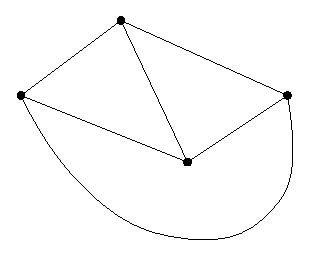
\includegraphics[width=0.2\textwidth]{GATL2_6.eps}
	\caption{Плоский граф.}
	\label{2_6}
\end{figure}

\begin{theorem}
	Если существует (непрерывное) вложение графа в плоскость, то существует и такое его вложение в плоскость, что его ребра изобразятся ломанными.
\end{theorem}
\begin{rem}
	Есть более сильное утверждение про отрезки, но оно нам не понадобится. Также отметим, что доказательство не будет состоять из попытки измененеия вложения графа на одном ребре так, чтобы на этом ребре мы получили ломанную. Это не получится из-за эффекта того, что при подходе к вершине ребра эти непрерывные кривые могут вести себя довольно сложным образом. Например, как $x \sin{\tfrac{1}{x}}$.
\end{rem}
\begin{proof}
	Доказательство будет состоять из нескольких шагов. Для простоты, пусть граф $G$ не имеет петель. По условию у нас есть некоторое вложение графа:
	\begin{enumerate}[label ={\arabic*)}]
		\item (\uline{\textbf{Изменение вложения в окрестности вершин}}):
		
		Для каждой вершины $v$ графа $G$ рассмотрим замкнутый круг $D_v$ так, чтобы:
		\begin{enumerate}[label ={(\arabic*)}]
			\item Эти круги не пересекались;
			\item Каждый круг $D_v$ не пересекался с ребрами, не содержащими вершину $v$;
		\end{enumerate}
		Пункт $(2)$ возможен в силу утверждения, что образ непрерывной кривой это замкнутое подмножество плоскости $\Rightarrow$ вершина $v$ не принадлежит этой кривой, поэтому можно выбрать какую-то её окрестность, которая с образом этой непрерывной кривой не пересекается. Уменьшив эту окрестность, можно в ней выбрать замкнутый круг. Если круги как-то пересекаются, то в силу того, что у нас конечное число вершин, можно их ещё раз уменьшить.
		\begin{figure}[H]
			\centering
			\includegraphics[width=0.4\textwidth]{GATL2_7.eps}
			\caption{Построение кругов $D_v$.}
			\label{2_7}
		\end{figure}
		Для каждого ребра $e$, которое имеет вершину $v$ одной из концевых точек, рассмотрим его как непрерывную кривую идущую из какой-то вершины $w$ в вершину $v \Rightarrow$ по лемме о первой точке на этой кривой будет первая точка, принадлежащая $D_v$. Изменем вложение для этого ребра на отрезке после первой точки ``на радиус'': уберём всё, что было после первой точки и соединим её с центром круга (получив таким образом радиус).
		\begin{figure}[H]
			\centering
			\includegraphics[width=0.8\textwidth]{GATL2_8.eps}
			\caption{Изменение вложения ``на радиус''.}
			\label{2_8}
		\end{figure}
		Сделаем так для всех рёбер и для всех вершин.
		\item (\uline{\textbf{Изменение вложения на ``средних'' частях рёбер}}):
		
		Рассмотрим часть ребра вне кругов $D_v$ и $D_w$, как среднюю часть $\Rightarrow$ это непрерывная кривая $\gamma \colon [a,b] \to \MR^2$. Рассмотрим множество: $T = \{t \in[a,b] \mid l(t) \colon \gamma(a) \to \gamma(t)\}$, в котором $\gamma(a)$ можно соединить ломанной кривой $l(t)$ с $\gamma(t)$ так, чтобы эта ломанная не имела самопересечений и не пересекала другие рёбра. $\exists \, t \in [a,b] \colon t \in T$, например? $a \in T \Rightarrow T \neq 0$. Далее, будем называть такую ломанную требуемой. Хотим доказать, что $b \in T$. 
		
		Очевидно, что $T \subset [a,b] \Rightarrow$ оно ограниченно. Докажем, что если $t_0 \in T$, то $(t_0 - \VE, t_0 + \VE) \subset T$ для некоторого $\VE> 0$, иными словами докажем, что $T$ - открытое подмножество отрезка. Пусть $t_0 \in T$, рассмотрим замкнутый круг с центром в $\gamma(t_0)$, который не пересекает другие рёбра и круги $D_v$, это возможно так как образы других рёбер - замкнутые подмножества в плоскости. Таким образом, по предположению существует требуемая ломанная, которая идёт до точки $\gamma(t_0)$. Тогда мы можем соединить $\gamma(a)$ с любой точкой круга $D_{\gamma(t_0)}$ с помощью требуемой ломанной, пройдя по ломанной из $\gamma(a)$ в $\gamma(t_0)$ до первой её точки в круге $D_{\gamma(t_0)}$ и дальше по отрезку, минуя любые самопересечения внутри круга.
		\begin{figure}[H]
			\centering
			\includegraphics[width=0.65\textwidth]{GATL2_9.eps}
			\caption{Построение ломанной до точки внутри круга с центром в $\gamma(t_0)$.}
			\label{2_9}
		\end{figure}
		С другой стороны, по определению непрерывности кривой для круга $D_{\gamma(t_0)}$ верно:
		$$
			\exists \, (t_0 - \VE, t_0 + \VE) \colon \gamma((t_0 - \VE, t_0 + \VE)) \subset D_{\gamma(t_0)}
		$$
		Таким образом, мы можем соединить требуемую ломанную с любой точкой этого интервала $\Rightarrow$ мы доказали желаемое: $(t_0 - \VE, t_0 + \VE) \subset T \Rightarrow T$ - открытое подмножество в $[a,b]$.
		
		Докажем (аналогично), что если $t_0 \not\in T$, то $\exists \, \VE > 0 \colon (t_0 - \VE, t_0 + \VE)\cap T = \VN$, то есть, что дополнение отрезка $[a,b]\setminus T$ тоже открыто. Пусть теперь $t_0 \not\in T$, рассмотрим для неё замкнутый круг и интервал вокруг этой точки. Если мы как-то смогли соединить требуемой ломанной $\gamma(a)$ с какой-то точкой из интервала $(t_0 - \VE, t_0 + \VE)$, то мы доходим до первой точки и далее идём до $\gamma(t_0)$.
		
		Докажем, что если $T \subset [a,b]$ и $([a,b]\setminus T) \subset [a,b]$ это открытые подмножества в $[a,b]$, то одно из них пусто. Рассмотрим:
		$$
			S = \{t \in [a,b] \mid [a,t] \subset T\}, \quad \sup\limits_{[a,b]}\{t \in [a,b] \mid [a,t] \subset T\} = c
		$$ 
		мы знаем, что $a \in T$ и следовательно будем идти по отрезку $[a,b]$, пока находимся в $T$ (может оказаться, что $a = c$). Пусть $c \in T \wedge c \neq b$, тогда $\exists \, \VE > 0 \colon (c - \VE, c+ \VE) \subset T$, а значит $c$ не является просто верхней гранью для $S \Rightarrow c \not\in T \vee c = b$.
		\begin{figure}[H]
			\centering
			\includegraphics[width=0.4\textwidth]{GATL2_10.eps}
			\caption{Нахождение точной верхней грани для $S$.}
			\label{2_10}
		\end{figure}
		 Аналогично, если $c \not\in T \Rightarrow c \in [a,b]\setminus T \Rightarrow \exists \, \VE > 0 \colon (c - \VE, c + \VE) \subset [a,b]\setminus T$, но тогда $c$ не является точной верхней гранью, поскольку $(c - \VE)$ - верхняя грань. Таким образом, единственный оставшийся вариант: $c = b$. Следовательно, мы всё доказали при предположении, что граф $G$ не имеет петель. 
		 
		 В случае, когда есть петли мы сначала рассмотрим граф без петель, затем, вспомнив про петли, мы можем в каждой вершине достроить сколько нам нужно петель в виде требуемых ломанных.
	\end{enumerate}
\end{proof}
\newpage

\begin{rem}
	Заметим, что далее мы будем пользоваться этой теоремой в переформулированном виде: если не существует вложения графа в плоскость, при котором он изображается ломанными, то граф не планарный. Поэтому, чтобы доказать, что какой-то граф не планарный, то достаточно доказать, что не существует вложения этого графа в плоскость при котором его рёбра изображаются ломанными.
\end{rem}

\subsection*{Теорема Жордана}
Пусть $G$ - плоский граф, $|V|$ - число его вершин, $|E|$ -  число его рёбер. Введём отношение эквивалентности точек. 
\begin{defn}
	Для любого подмножества $A$ плоскости отношение: точки $P,Q \in A$ можно соединить непрерывной кривой, лежащей в $A$, является \uwave{отношением эквивалентности}. Соответствующие классы эквивалентности называются \uwave{компонентами линейной связности} множества $A$ или просто компонентами.
\end{defn}
\begin{rem}
	Будем пользоваться свойствами отношения эквивалентности, которые рассматриваются на математическом анализе.
\end{rem}

\begin{figure}[H]
	\centering
	\includegraphics[width=0.15\textwidth]{GATL2_11.eps}
	\caption{Отношение эквивалентности для $P$ и $Q$ внутри $A$.}
	\label{2_11}
\end{figure}
Рассмотрим для нашего графа множество $\MR^2 \setminus G$. Это множество будет иметь какое-то количество компонент линейной связности (проще говоря, то количество областей на которые граф разбивает плоскость). Обозначим $|\Gamma|$ - количество компонент множества $\MR^2 \setminus G$.
\begin{figure}[H]
	\centering
	\includegraphics[width=0.25\textwidth]{GATL2_12.eps}
	\caption{Граф $G$.}
	\label{2_12}
\end{figure}
Рассматривая простешие графы ($1$ вершина, $1$ ребро $\Rightarrow$ замкнутая непрерывная кривая), можно заметить, что все эти величины $|\Gamma|, \, |V|, \, |E|$ как-то связаны. Возникает вопрос на сколько частей может разбивать плоскость граф в виде непрерывной кривой. Ответ на этот вопрос даёт теорема Жордана. Отметим, что для некоторых простых кривых мы можем дать ответ, что замкнутая вложенная кривая разбивает плоскость на две части и оказывается, что отсюда уже можно вывести теорему Жордана в общем виде, что совсем не очевидно.
 
\end{document}